\documentclass[11pt,a4paper,openany]{report}
\usepackage[T1]{fontenc}
\usepackage[utf8]{inputenc}
\usepackage{lmodern}
\usepackage{microtype}
\usepackage{amsmath,amssymb,amsthm,mathtools,bm}
\usepackage{booktabs,array,longtable,tabularx}
\usepackage{xcolor}
\usepackage[margin=24mm,headheight=23pt]{geometry}
\usepackage{enumitem}
\usepackage{fancyhdr}
\usepackage{fancyvrb}
\usepackage{graphicx}
\usepackage{url}
\usepackage{xurl}
\usepackage{hyperref}

\definecolor{finblue}{HTML}{1F5A99}
\definecolor{fingreen}{HTML}{19733A}
\definecolor{finorange}{HTML}{D55E00}
\definecolor{finred}{HTML}{A61B1B}
\definecolor{finviolet}{HTML}{6A3D9A}

\hypersetup{
  unicode=true,
  colorlinks=true,
  linkcolor=finblue,
  citecolor=fingreen,
  urlcolor=finblue,
  pdftitle={FIN Programs 91--100: Critical Scaling, Nonlocal Continuum Structure, and Operational Completion Tests},
  pdfauthor={Krzysztof Żuchowski},
  pdfsubject={Schur nonclosure, critical scaling, nonlocal continuum limits, process tensors, and damping completion},
  pdfkeywords={FIN, Schur complement, renormalization, graphon, nonlocal operator, process tensor, information thermodynamics}
}

\pagestyle{fancy}
\fancyhf{}
\fancyhead[L]{\small FIN Programs 91--100}
\fancyhead[R]{\small Release 10.10}
\fancyfoot[C]{\thepage}
\setlength{\parindent}{0pt}
\setlength{\parskip}{0.55em}
\setlist{nosep,leftmargin=2em}
\setcounter{tocdepth}{2}
\setcounter{secnumdepth}{3}
\emergencystretch=3em

\newcommand{\one}{\bm 1}
\newcommand{\C}{\mathbb C}
\newcommand{\R}{\mathbb R}
\newcommand{\Z}{\mathbb Z}
\newcommand{\statusProven}{\textcolor{fingreen}{[Proven]}}
\newcommand{\statusComputer}{\textcolor{fingreen}{[Proven, computer-assisted]}}
\newcommand{\statusStrong}{\textcolor{finblue}{[Strong evidence]}}
\newcommand{\statusModerate}{\textcolor{finviolet}{[Moderate evidence]}}
\newcommand{\statusConditional}{\textcolor{finorange}{[Conditional]}}
\newcommand{\statusRefuted}{\textcolor{finred}{[Refuted]}}
\newcommand{\statusOpen}{\textcolor{finviolet}{[Open]}}

\begin{document}
\hypersetup{pageanchor=false}
\begin{titlepage}
\centering
\vspace*{9mm}
{\Large\bfseries FIN Research Monograph --- Release 10.10\par}
\vspace{11mm}
{\Huge\bfseries FIN Programs 91--100\par}
\vspace{6mm}
{\Large Critical Scaling, Nonlocal Continuum Structure,\\
and Operational Completion Tests\par}
\vspace{17mm}
{\Large Krzysztof \.Zuchowski\par}
\vspace{2mm}
{\normalsize Independent Researcher --- Fractal Information Theory Project\par}
\vspace{2mm}
{\normalsize ORCID: \href{https://orcid.org/0009-0002-0909-3613}{0009-0002-0909-3613}\par}
\vspace{10mm}
{\large 27 July 2026\par}
{\normalsize Publication --- Preprint; record version 1.0.0\par}
\vfill
\begin{minipage}{0.88\textwidth}
\small
\textbf{Scope.} Ten executed studies of strict-kernel Schur nonclosure,
critical scaling, graphon continuum limits, long-range propagation,
adaptive quotient structure, selector-source provenance, process-tensor
design, feedback thermodynamics, data acquisition, and the
legacy--strict damping-completion atom.

\medskip
\textbf{Central theorem.} A tail-controlled scale-invariant spectral ratio
proves that the fixed-mass strict lattice family is not closed, even up to
scalar normalization, under alternating-site Schur reduction.

\medskip
\textbf{Guardrail.} No strict selector, physical-unit source, Lorentz closure,
legacy role transfer, completed legacy--strict bridge, role-bearing
\(L_{\mathrm{total}}\), or external physical validation is claimed.

\medskip
\textbf{License.} Creative Commons Attribution 4.0 International (CC BY 4.0).
\end{minipage}
\vfill
\end{titlepage}
\hypersetup{pageanchor=true}

\pagenumbering{roman}
\chapter*{Publication statement}
\addcontentsline{toc}{chapter}{Publication statement}
This release reports Programs 91--100 and recommends Programs 101--112.
Theorem-level statements, computer-assisted certificates, numerical evidence,
conditioned operational models, failed inferences, and open obligations are
labeled separately.

\tableofcontents
\clearpage
\pagenumbering{arabic}

\section{Confidence convention}

\begin{itemize}
\item 
\textbf{\statusProven{}} analytic theorem or exact finite algebra under the stated definitions.

\item 
\textbf{\statusComputer{}} exact finite computation joined to an explicit rigorous remainder bound.

\item 
\textbf{\statusStrong{}} reproducible computation with a large margin and frozen protocol.

\item 
\textbf{\statusConditional{}} exact only after declared operational or physical inputs are supplied.

\item 
\textbf{\statusRefuted{}} a declared claim contradicted inside its stated scope.

\item 
\textbf{\statusOpen{}} neither proved nor rigorously falsified.

\end{itemize}

The nadsoliton ontology is retained as a project premise, not promoted to experimentally established physics. The strict kernel remains the strict working object; the legacy kernel remains an intermediate bridge object.

\par\medskip\hrule\medskip

\chapter{Abstract}

This monograph executes FIN Research Programs 91--100. It starts from the strict/\allowbreak{}legacy kernel split and from the exact harmonic-alias Schur law obtained in Programs 81--90. Its central purpose is to replace suggestive large-matrix trends with sharper mathematical statements and then to continue the operational reconstruction without promoting imported physics to strict FIN output.

The principal result is a computer-assisted nonclosure theorem for the infinite-lattice strict profile at fixed mass \(m^2=1/4\). An explicit \(d^{-1.8}\) tail estimate encloses two scale-invariant spectral ratios before and after alternating-site Schur reduction. The intervals are disjoint by more than \(0.1497\). Therefore no scalar field or operator normalization can return the reduced precision to the same fixed strict family. This converts the finite-size plateau of Program 81 into a tail-controlled theorem in a declared realization.

Two different continuum routes are then separated. A nearest-neighbour local precision admits the exact renormalization law

\[
\frac{m'}{c'}=r(r+4),\qquad r=\frac{m}{c},
\]

so a finite local continuum mass requires the critical prescription \(r_N=\mu^2/N^2\) and a factor-two operator renormalization on the massless kinetic term. By contrast, the coordinate-rescaled dense strict profile converges at first order to a bounded circle-convolution operator. Its eigenvalues tend to \(m^2+1\) at high Fourier mode rather than growing as \(k^2\). It is a valid nonlocal continuum theory, not a local Laplacian field theory.

For the lattice strict profile, the coupling mass outside radius \(R\) obeys a polynomial \(R^{-0.8}\) bound. Hence both unitary and diffusive propagators are approximable by finite-range dynamics, but the natural error is polynomial, not a strict causal cone. The adaptive moment law is proven to be a projected gradient flow on a chosen operator subspace, while its stronger regulator-free quotient interpretation is refuted for the tested nonlinear functional. The P2772 self-learning candidate is independently reproduced: both frozen kernel tuples have nonzero gradients.

The post-P2721 selector artifacts are revalidated and no strict signed source is admitted. A noisy two-slot process-tensor design is optimized, an apparatus-inclusive feedback identity is completed, and a preregistered external-data acquisition calculation is supplied. Finally, the smallest pointwise damping-completion atom

\[
C_{\mathrm{damp}}(d)
=\frac{1+\beta_{\mathrm{tors}}d}{1+\beta d^{9/5}}
\]

is constructed. It is mathematically necessary for the two frozen damping envelopes and has asymptotic degree \(-4/5\), but it is target-coded and lacks a FIN source theorem.

No result closes \(QW\text{-}2191\), generates dimensional standards, proves Lorentz invariance, completes the legacy-to-strict bridge, transfers legacy physical roles, promotes a role-bearing \(L_{\mathrm{total}}\), or supplies external physical evidence.

\par\medskip\hrule\medskip

\chapter{Executive summary}

\section{The ten executed programs}

\begin{center}
\begingroup\small
\setlength{\tabcolsep}{3.5pt}
\renewcommand{\arraystretch}{1.16}
\begin{longtable}{@{}p{0.075\textwidth}p{0.246\textwidth}p{0.311\textwidth}p{0.228\textwidth}@{}}
\toprule
\textbf{Program} & \textbf{Question} & \textbf{Result} & \textbf{Confidence} \\
\midrule
\endhead
91 & Is the strict lattice nonclosure only a finite-size effect? & No. A tail-controlled two-mode ratio certificate proves nonclosure at \(m^2=1/4\). & \textbf{Proven, computer-assisted} \\
92 & What tuning produces the local nearest-neighbour continuum route? & \(r'=r(r+4)\), \(r_N=\mu^2/N^2\), and factor-two kinetic renormalization. & \textbf{Proven} \\
93 & What is the natural continuum object of coordinate-rescaled strict matrices? & A bounded nonlocal convolution/\allowbreak{}graphon operator, not a local Laplacian. & \textbf{Proven in the continuum formulation; strong numerical convergence} \\
94 & How fast does influence outside a finite range decay? & Polynomially: \(R^{1-\eta}=R^{-0.8}\); no strict finite cone follows. & \textbf{Proven bound; strong numerical check} \\
95 & Is adaptive FIN dynamics a regulator-free quotient gradient flow? & It is a projected gradient flow after a subspace is chosen; quotient invariance fails for the tested functional. & \textbf{Proven/\allowbreak{}refuted in declared scope} \\
96 & Do post-P2721 artifacts supply the missing chiral source? & No accepted source satisfies formula, sign, provenance, polarity, and gauge criteria. & \textbf{Provenance result} \\
97 & Which noisy two-slot experiment best separates wave and diffusion? & Full-site records at half-time \(0.97244\) maximize the tested worst-case divergence. & \textbf{Conditional numerical result} \\
98 & Does feedback yield free work when the apparatus is included? & No. \(W_{\mathrm{complete}}-\Delta F=H(Y\mid X)\ge0\). & \textbf{Proven operational identity} \\
99 & How many records are sufficient under the Program 97 model? & Chernoff bounds give 14, 23, 36, 49 shots for error bounds \(0.05,0.01,0.001,10^{-4}\). & \textbf{Conditional model-based bound} \\
100 & What is the minimal damping atom needed in the legacy-to-strict bridge? & An exact multiplier of asymptotic degree \(-4/5\); its source remains absent. & \textbf{Proven necessity; source open} \\
\bottomrule
\end{longtable}
\endgroup
\end{center}

\section{The central scientific correction}

Programs 81--90 found that dense-row Frobenius convergence can be a dilution artifact. Programs 91--100 now show that the repository contains two mathematically legitimate but inequivalent continuum questions:

\begin{enumerate}
\item 
\textbf{Local critical route.} Start from a local finite-range precision, tune the mass toward a critical surface, and renormalize the kinetic coefficient.

\item 
\textbf{Dense nonlocal route.} Rescale the kernel coordinate to a fixed compact domain and obtain a bounded integral operator.

\end{enumerate}

These routes must not be conflated. The first can produce a local differential operator but needs scale-dependent tuning that the frozen strict kernel does not generate. The second is naturally generated by dense strict discretizations but remains nonlocal and spectrally bounded.

\section{Strongest positive statement}

The strict kernel has a mathematically coherent interpretation as a long-range jump profile and as a compact-domain convolution profile. Both generate the same pair of temporal semantics,

\[
U_t=e^{-itA},
\qquad
P_t=e^{-tA},
\]

once a positive self-adjoint precision \(A\) is defined. The wave/\allowbreak{}diffusion duality is exact operator mathematics.

\section{Strongest negative statement}

The frozen strict lattice family is not an exact scalar-normalized fixed family of alternating-site Gaussian elimination at \(m^2=1/4\). The observed failure is not explained by the finite sizes used in Program 81.

\section{What remains missing for physics}

The following inputs remain independent of the kernel:

\begin{itemize}
\item 
a dimensional clock and action scale;

\item 
a preparation rule;

\item 
an admissible measurement instrument;

\item 
a detector and calibration map;

\item 
an environment/\allowbreak{}bath;

\item 
a state law, including any Born-type rule;

\item 
a strict orientation/\allowbreak{}polarity source;

\item 
an independently acquired dataset.

\end{itemize}

Thus the operator supports an operational theory \textbf{conditioned on} these inputs. It does not generate them.

\par\medskip\hrule\medskip

\chapter{Scope and claim discipline}

\section{Kernel split}

The analysis keeps the two frozen objects distinct:

\[
K_{\mathrm{legacy,ont}}(d)
=
\alpha_{\mathrm{geo}}
\frac{\cos(\pi d/4+\pi/6)}
{1+\beta_{\mathrm{tors}}d},
\qquad
\alpha_{\mathrm{geo}}=4\ln2,
\quad
\beta_{\mathrm{tors}}=0.01,
\]

and

\[
K_{\mathrm{strict,gate}}(d)
=
\frac{\cos(0.18575d+0.16250)}
{1+d^{1.8}}.
\]

The legacy kernel is treated as an intermediate ontological bridge kernel. The strict kernel is treated as the later completed/\allowbreak{}enriched working kernel only where an explicit completion component has been constructed. No legacy physical-role formula is transferred to the strict kernel.

\section{Ontology}

The ontology used in this report is:

\[
\text{nadsoliton}
\longrightarrow
\text{light}
\longrightarrow
\text{matter}
\longrightarrow
\text{emergent observer}.
\]

The nadsoliton itself is the primordial information in a solitonic state. There is no separate informational substrate underneath it. This ontological statement does not by itself supply a metric, physical unit, selector, or measurement law.

\section{Detailed confidence labels}

The labels have the following meanings.

\begin{itemize}
\item 
\textbf{\statusProven{}} An analytic argument or exact algebraic identity is given.

\item 
\textbf{\statusComputer{}} A finite or truncated calculation is joined to an explicit rigorous remainder bound.

\item 
\textbf{\statusStrong{}} Stable numerical convergence supports a standard analytic identification, but a complete formal error proof is not included.

\item 
\textbf{\statusConditional{}} The result is exact after stated operational inputs are supplied.

\item 
\textbf{\statusRefuted{}} A declared claim fails by theorem or explicit counterexample.

\item 
\textbf{\statusOpen{}} No theorem or adequate evidence settles the claim.

\end{itemize}

\section{Reproducibility}

All reported numbers are generated by \path{fin_programs_91_100_critical_nonlocal_operational.py}. Seventeen regression and theorem-invariant tests are in test\_\path{fin_programs_91_100_critical_nonlocal_operational.py}. Machine-readable results are stored in \path{FIN_Programs_91_100_Critical_Nonlocal_Operational_Results.json}.

\par\medskip\hrule\medskip

\chapter{Common operator setup}

Let \(a_d\ge0\) be a symmetric summable profile on the integer lattice:

\[
Z=2\sum_{d\ge1}a_d,
\qquad
p_{\pm d}=\frac{a_d}{Z}.
\]

The associated Markov convolution \(P\) and positive precision are

\[
(Pf)_x=\sum_{d\ne0}p_d f_{x-d},
\qquad
A=m^2I+I-P.
\]

Their Fourier symbols are

\[
\widehat p(q)=2\sum_{d\ge1}\frac{a_d}{Z}\cos(qd),
\qquad
\lambda(q)=m^2+1-\widehat p(q).
\]

Because \(-1\le\widehat p(q)\le1\),

\[
m^2\le\lambda(q)\le m^2+2.
\]

Consequently \(A\) is bounded, positive, and self-adjoint for \(m^2>0\). Both

\[
U_t=e^{-itA}
\]

and

\[
P_t=e^{-tA}
\]

are functions of this same spectral object. This shared generator is proven mathematics. Calling either parameter a physical time requires an additional clock calibration.

For Programs 91 and 94,

\[
a_d
=
\frac{|\cos(\omega_sd+\phi_s)|}{1+d^\eta},
\qquad
\eta=1.8.
\]

The absolute value is necessary for a jump/\allowbreak{}Dirichlet interpretation. It is not an assertion that the signed strict kernel itself is a Markov weight.

\par\medskip\hrule\medskip

\chapter{Program 91 --- Tail-certified strict-lattice nonclosure}

\section{Objective}

Program 81 found a persistent large-\(N\) defect after alternating-site Schur reduction. Program 91 asks whether this can be turned into a theorem about the infinite strict lattice profile rather than a finite-size observation.

\section{Exact harmonic-alias law}

Split the lattice into retained even sites and eliminated odd sites. For a translation-invariant Gaussian precision, the two fine Fourier modes that alias to one coarse mode are combined by a harmonic mean:

\[
\lambda_{\mathrm{S}}(\theta)
=
\frac{
2\lambda(\theta/2)\lambda(\theta/2+\pi)
}{
\lambda(\theta/2)+\lambda(\theta/2+\pi)
}.
\]

This identity is exact. It is the Fourier representation of the Schur complement.

\section{A scalar-normalization invariant}

Any scalar field or operator renormalization multiplies the complete symbol by one positive constant. Therefore the ratio

\[
R=\frac{\lambda(0)}{\lambda(\pi)}
\]

is invariant under every such normalization.

For the native family,

\[
R_{\mathrm{native}}
=
\frac{m^2}{m^2+1-\widehat p(\pi)}.
\]

For the retained Schur operator, coarse \(\theta=0\) aliases fine \(0,\pi\), while coarse \(\theta=\pi\) aliases fine \(\pi/2,3\pi/2\). Reflection symmetry gives \(\lambda(3\pi/2)=\lambda(\pi/2)\), hence

\[
R_{\mathrm{Schur}}
=
\frac{
2m^2\lambda(\pi)/(m^2+\lambda(\pi))
}{
\lambda(\pi/2)
}.
\]

If these ratios differ, scalar-normalized family closure is impossible.

\section{Rigorous tail control}

Truncate the normalization at \(D=10^6\):

\[
Z_D=2\sum_{d=1}^{D}a_d.
\]

Since \(a_d\le d^{-\eta}\),

\[
0\le Z-Z_D
\le
\frac{2D^{1-\eta}}{\eta-1}
=3.962232981152781\times10^{-5}.
\]

The computed partial normalization is

\[
Z_D=1.9676797946362259.
\]

If \(N_D(q)\) is the truncated Fourier numerator, its missing tail has absolute value no larger than the normalization tail. A direct quotient estimate gives

\[
\left|
\widehat p(q)-\frac{N_D(q)}{Z_D}
\right|
\le
\frac{2(Z-Z_D)}{Z_D}
\le
4.027314801883502\times10^{-5}.
\]

This bound is applied independently at \(q=\pi\) and \(q=\pi/2\).

\section{Certified result}

At \(m^2=1/4\), the resulting enclosures are

\[
R_{\mathrm{native}}
\in
[0.1568166565,\ 0.1568245799],
\]

and

\[
R_{\mathrm{Schur}}
\in
[0.3065726598,\ 0.3065922757].
\]

The disjoint-interval margin is

\[
0.1497480799.
\]

\begin{figure}[htbp]
\centering
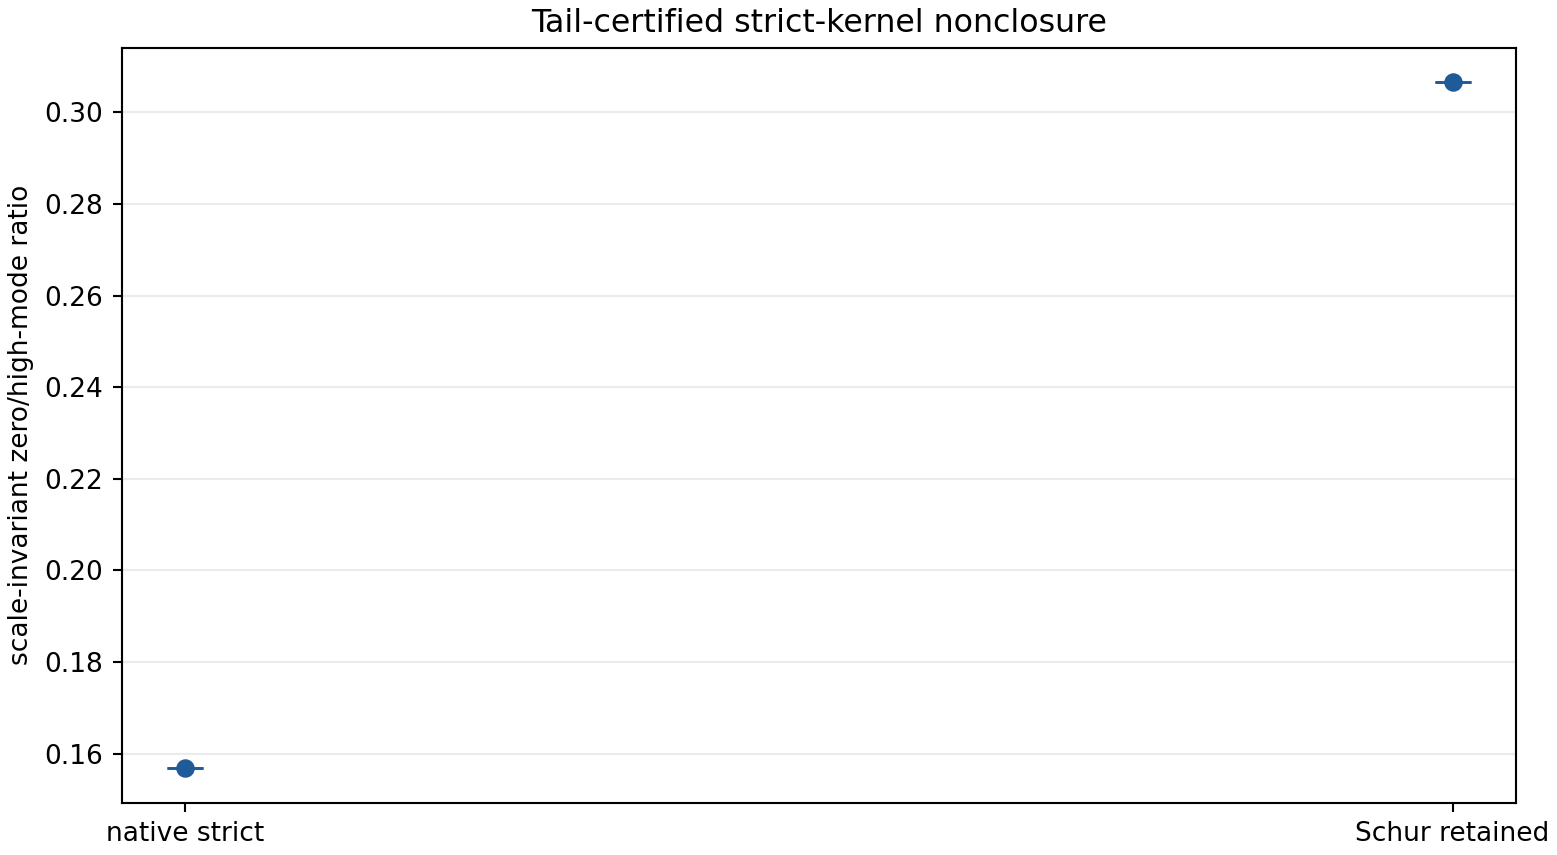
\includegraphics[width=0.92\textwidth]{FIN_Programs_91_100_Critical_Nonlocal_Operational_Figures/program91_strict_nonclosure_certificate.png}
\caption{Tail-certified separation of the native and Schur scale-invariant spectral ratios.}
\end{figure}


\section{Theorem}

\textbf{Theorem 91.1 --- fixed-mass scalar-normalized nonclosure. \statusComputer{}}

For the normalized infinite-lattice absolute strict profile

\[
a_d=\frac{|\cos(0.18575d+0.16250)|}{1+d^{1.8}},
\]

with precision \(A=\frac14 I+I-P\), one alternating-site Schur step is not a scalar multiple of the native strict precision family.

\textbf{Proof.} The exact harmonic-alias law gives the retained ratio. The displayed tail bound encloses both native and retained scale-invariant ratios in disjoint intervals. Scalar multiplication cannot change either ratio. Therefore no scalar multiplication identifies the two symbols. \(\square\)

\section{Falsification boundary}

The theorem does not exclude:

\begin{itemize}
\item 
a running mass;

\item 
running \(\omega,\phi,\beta,\eta\);

\item 
new counterterms;

\item 
a non-alternating coarse map;

\item 
an approximate effective flow;

\item 
a different signed-to-positive operator construction.

\end{itemize}

It does exclude the stronger statement that the frozen fixed-mass strict lattice precision is already an exact scalar-normalized Schur fixed family.

\par\medskip\hrule\medskip

\chapter{Program 92 --- Critical tuning and field rescaling}

\section{Objective}

If the frozen strict lattice route is not an exact fixed family, can a smaller local model show precisely what extra data are required for a local continuum limit?

\section{Nearest-neighbour precision}

Consider

\[
(Af)_n
=
mf_n+c(2f_n-f_{n-1}-f_{n+1}),
\qquad
m\ge0,\ c>0.
\]

Its symbol is

\[
\lambda(q)=m+2c(1-\cos q).
\]

Eliminating odd sites yields another nearest-neighbour precision. Direct block elimination gives

\[
c'=\frac{c^2}{m+2c},
\]

and

\[
m'=\frac{m(m+4c)}{m+2c}.
\]

Thus, for the dimensionless ratio \(r=m/c\),

\[
r'=r(r+4).
\]

\section{Fixed points}

On \(r\ge0\), the fixed-point equation

\[
r=r(r+4)
\]

has only

\[
r=0.
\]

The massless local Laplacian is therefore the nonnegative finite fixed point of the shape map. At \(m=0\),

\[
c'=\frac c2.
\]

The shape is fixed, but its coefficient is not. Multiplying the coarse operator by

\[
Z_A=2
\]

restores the kinetic coefficient.

\section{Critical finite-mass scaling}

Let a circle of fixed macroscopic size be discretized with \(N\) sites and set

\[
r_N=\frac{\mu^2}{N^2}.
\]

After one decimation,

\[
r_N'
=
4r_N+r_N^2.
\]

The target value on \(N/2\) sites is

\[
r_{N/2}=4r_N.
\]

Therefore

\[
r_N'-r_{N/2}=r_N^2,
\]

and the relative defect is exactly

\[
\frac{r_N^2}{4r_N}
=
\frac{\mu^2}{4N^2}.
\]

\begin{figure}[htbp]
\centering
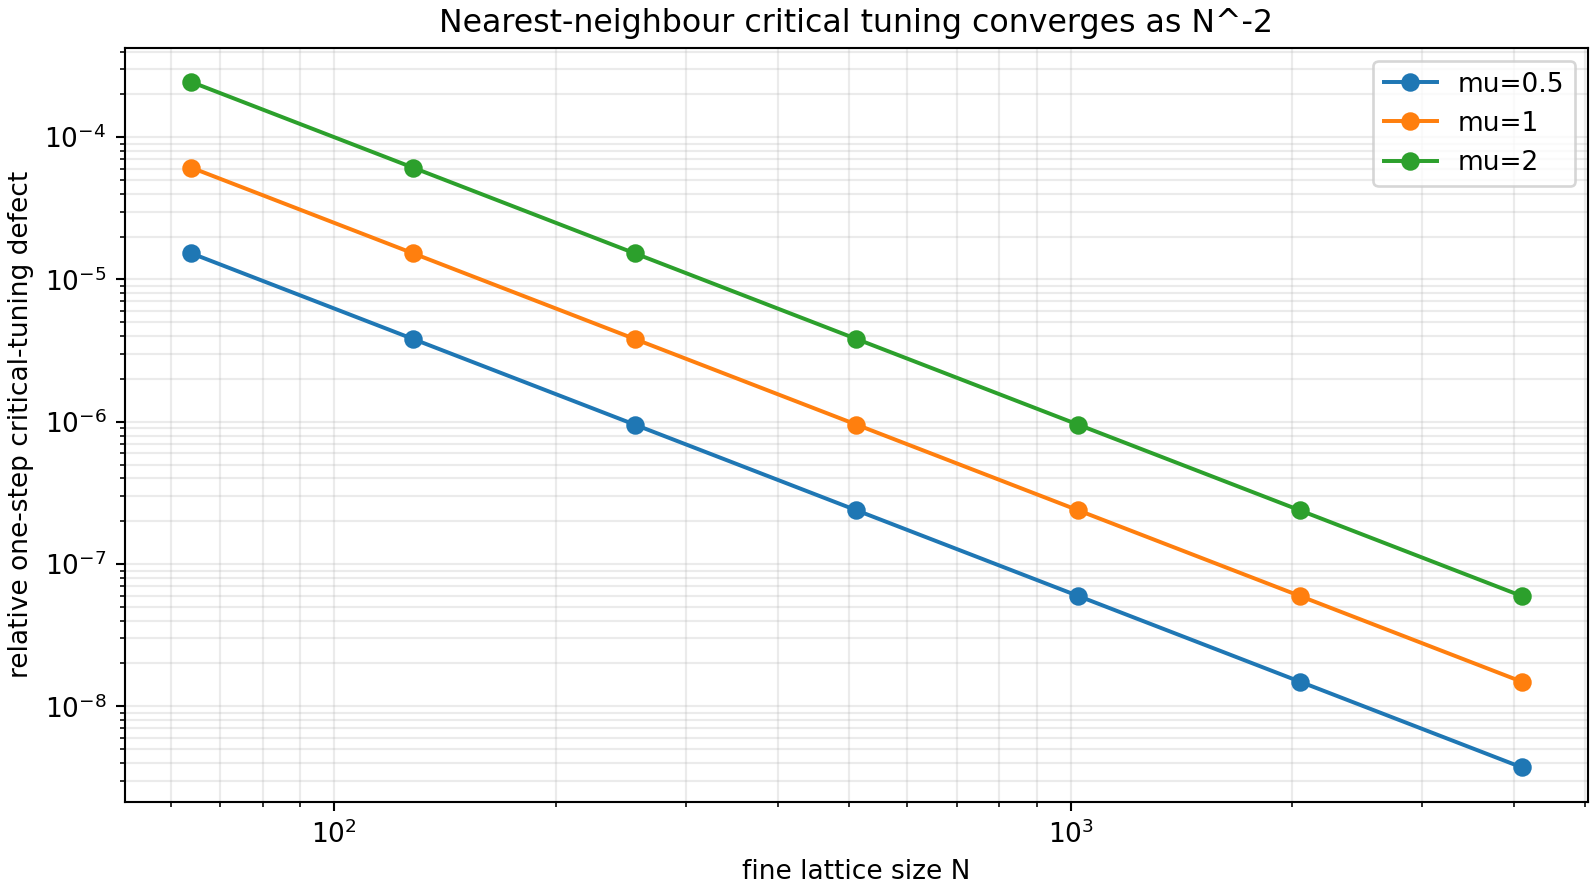
\includegraphics[width=0.92\textwidth]{FIN_Programs_91_100_Critical_Nonlocal_Operational_Figures/program92_critical_tuning.png}
\caption{Exact nearest-neighbour critical-tuning defect and its \(N^{-2}\) relative rate.}
\end{figure}


\section{Result}

\textbf{Theorem 92.1 --- local critical prescription. \statusProven{}}

A nearest-neighbour massive continuum route under alternating decimation requires both:

\begin{enumerate}
\item 
approach to the massless critical surface as \(m/c=O(N^{-2})\);

\item 
a factor-two operator normalization per decimation in the massless kinetic sector.

\end{enumerate}

Neither prescription follows merely from giving a frozen distance kernel.

\section{Interpretation}

This is the smallest explicit model of the missing renormalization data. It clarifies why "one operator at one resolution" is not yet a continuum field theory. A continuum theory requires a family indexed by resolution and a rule for how parameters and fields transform.

\par\medskip\hrule\medskip

\chapter{Program 93 --- The natural dense limit is a nonlocal graphon operator}

\section{Objective}

Program 81 found that coordinate-rescaled dense strict matrices have vanishing Frobenius defects but persistent uniform symbol defects. Program 93 identifies the actual continuum object.

\section{Continuum profile}

On the unit circle, let

\[
g(x)
=
\left|
K_{\mathrm{strict,gate}}
\bigl(\operatorname{dist}_{S^1}(0,x)\bigr)
\right|.
\]

Let

\[
Z=\int_0^1g(x)\,dx
\]

and define

\[
(Tf)(x)
=
\frac1Z
\int_0^1
g(x-y)f(y)\,dy.
\]

Then

\[
A=m^2I+I-T
\]

is a bounded self-adjoint convolution precision.

\section{Spectrum}

The Fourier basis diagonalizes \(T\):

\[
T e_k=\widehat g_k e_k,
\qquad
e_k(x)=e^{2\pi ikx}.
\]

By the Riemann--Lebesgue lemma,

\[
\widehat g_k\longrightarrow0.
\]

Therefore

\[
\lambda_k(A)
=
m^2+1-\widehat g_k
\longrightarrow
m^2+1.
\]

This is incompatible with a local second-order Laplacian, whose eigenvalues grow as \(k^2\).

\section{Numerical convergence}

The first 33 discrete Fourier coefficients were compared with a \(2^{20}\)-point midpoint continuum quadrature.

\begin{center}
\begingroup\small
\setlength{\tabcolsep}{3.5pt}
\renewcommand{\arraystretch}{1.16}
\begin{longtable}{@{}p{0.420\textwidth}p{0.420\textwidth}@{}}
\toprule
\textbf{\(N\)} & \textbf{maximum error, modes \(0,\ldots,32\)} \\
\midrule
\endhead
128 & \(8.7870\times10^{-3}\) \\
256 & \(4.3727\times10^{-3}\) \\
512 & \(2.1812\times10^{-3}\) \\
1024 & \(1.0893\times10^{-3}\) \\
2048 & \(5.4433\times10^{-4}\) \\
4096 & \(2.7208\times10^{-4}\) \\
8192 & \(1.3602\times10^{-4}\) \\
\bottomrule
\end{longtable}
\endgroup
\end{center}

The fitted rate is

\[
N^{-1.00199}.
\]

Selected precision eigenvalues at \(m^2=1/4\) are

\[
\lambda_0=0.25,
\qquad
\lambda_1=1.19358,
\qquad
\lambda_{4096}=1.250000002.
\]

Moreover,

\[
\frac{\lambda_k-m^2}{(2\pi k)^2}
\]

falls from \(2.39\times10^{-2}\) at \(k=1\) to \(1.51\times10^{-9}\) at \(k=4096\).

\begin{figure}[htbp]
\centering
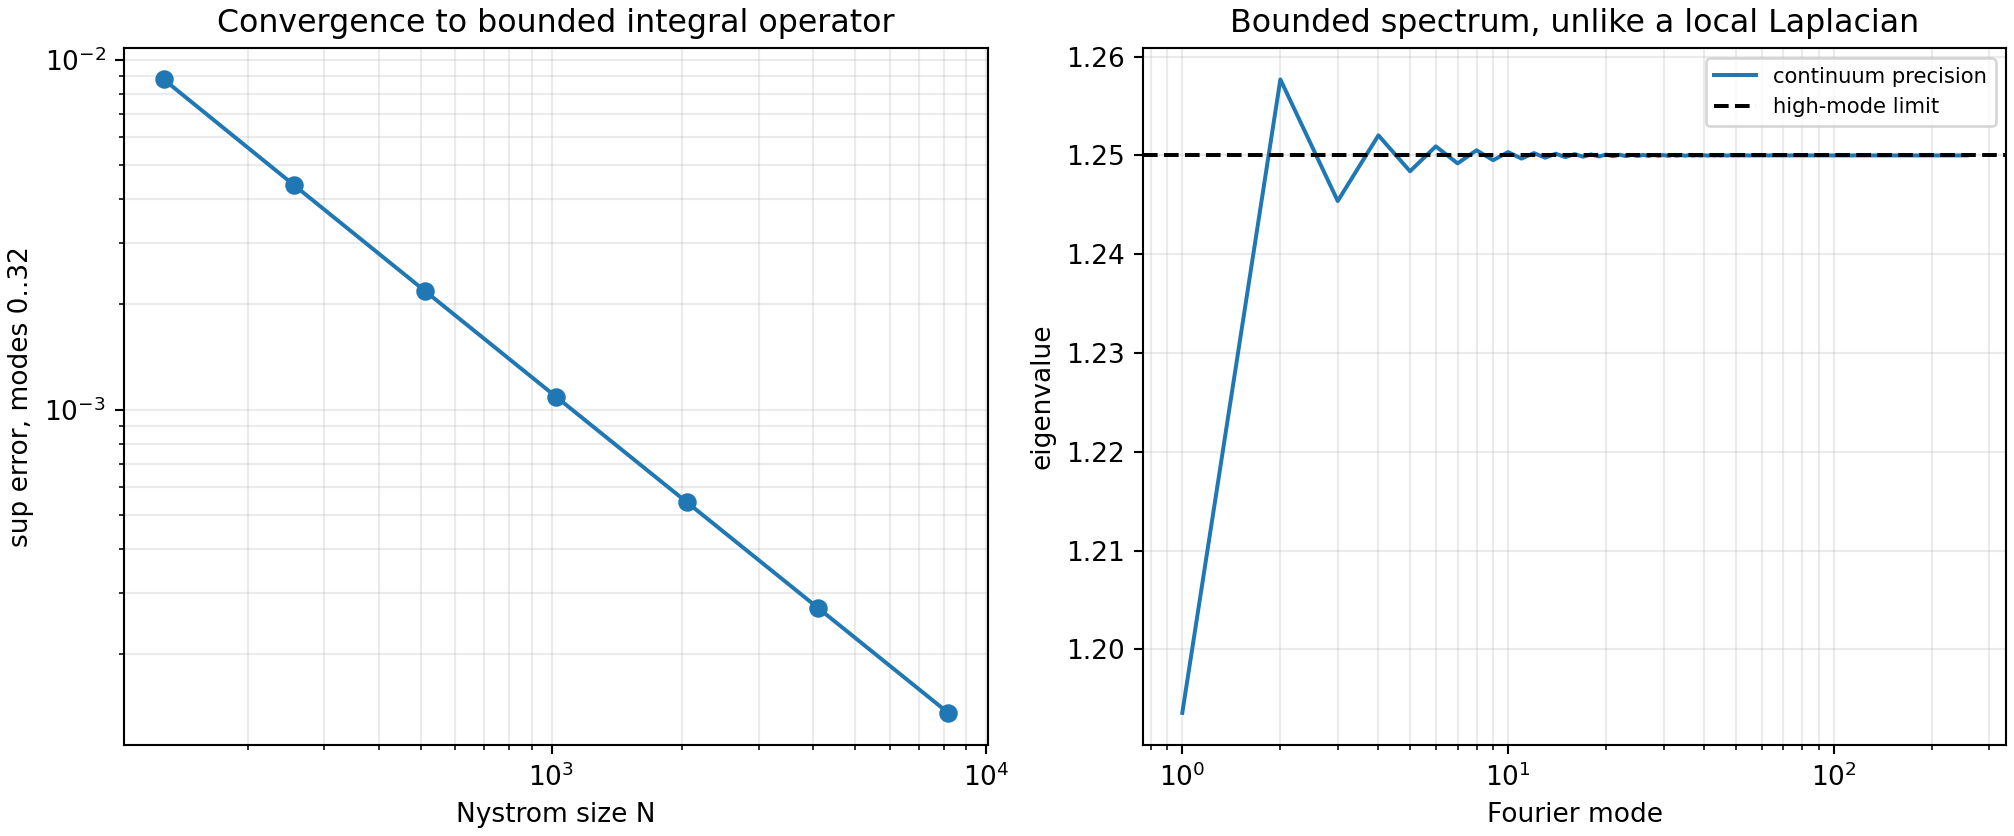
\includegraphics[width=0.92\textwidth]{FIN_Programs_91_100_Critical_Nonlocal_Operational_Figures/program93_graphon_continuum.png}
\caption{First-order discretization convergence and bounded high-mode continuum spectrum.}
\end{figure}


\section{Result}

\textbf{Theorem 93.1 --- continuum classification. [Proven, with strong numerical discretization evidence]}

The coordinate-rescaled dense strict matrices are Nyström discretizations of a bounded nonlocal convolution operator. Their natural high-frequency limit is bounded. They do not converge to a local Laplacian without an additional singular rescaling or counterterm construction.

\section{Physical boundary}

A nonlocal integral operator can be mathematically fundamental. It can also serve as a neural operator or graphon dynamics. But bounded nonlocality does not itself produce:

\begin{itemize}
\item 
a local spacetime metric;

\item 
a Lorentzian signature;

\item 
a finite propagation speed;

\item 
stress-energy;

\item 
canonical SI units.

\end{itemize}

\par\medskip\hrule\medskip

\chapter{Program 94 --- Polynomial propagation bounds}

\section{Objective}

Both \(e^{-itA}\) and \(e^{-tA}\) instantly use every nonzero matrix entry. The question is whether the long-range strict tail nevertheless supports a useful approximate locality statement.

\section{Tail mass}

For the normalized infinite profile, define

\[
\tau(R)
=
\sum_{|d|>R}p_d.
\]

Since \(a_d\le d^{-\eta}\),

\[
\tau(R)
\le
\frac{2}{Z(\eta-1)}R^{1-\eta}.
\]

For \(\eta=1.8\),

\[
\tau(R)=O(R^{-0.8}).
\]

The finite computation gives a fitted exponent

\[
-0.80143.
\]

Representative certified upper bounds are

\begin{center}
\begingroup\small
\setlength{\tabcolsep}{3.5pt}
\renewcommand{\arraystretch}{1.16}
\begin{longtable}{@{}p{0.420\textwidth}p{0.420\textwidth}@{}}
\toprule
\textbf{\(R\)} & \textbf{\(\tau(R)\) upper bound} \\
\midrule
\endhead
16 & \(8.6445\times10^{-2}\) \\
64 & \(2.9304\times10^{-2}\) \\
256 & \(9.5196\times10^{-3}\) \\
1024 & \(3.1692\times10^{-3}\) \\
4096 & \(1.0491\times10^{-3}\) \\
32768 & \(2.0479\times10^{-4}\) \\
\bottomrule
\end{longtable}
\endgroup
\end{center}

\section{Duhamel estimate}

Let \(L_R\) remove all edges longer than \(R\) without renormalizing the remaining edges. Then the discarded Laplacian has row mass \(\tau(R)\), and

\[
\|L-L_R\|\le2\tau(R).
\]

For the heat semigroup,

\[
e^{-tL}-e^{-tL_R}
=
-\int_0^t
e^{-(t-s)L}(L-L_R)e^{-sL_R}\,ds,
\]

so contractivity gives

\[
\|e^{-tL}-e^{-tL_R}\|
\le
2t\tau(R).
\]

The same argument with unitary factors yields

\[
\|e^{-itL}-e^{-itL_R}\|
\le
2|t|\tau(R).
\]

\section{Direct propagation witness}

On an \(8192\)-cycle at \(t=0.2\), the heat mass outside \(R\) decreases from \(2.84\times10^{-2}\) at \(R=8\) to \(8.89\times10^{-4}\) at \(R=512\). The wave probability outside the same radii decreases from \(1.19\times10^{-5}\) to \(3.53\times10^{-10}\).

\begin{figure}[htbp]
\centering
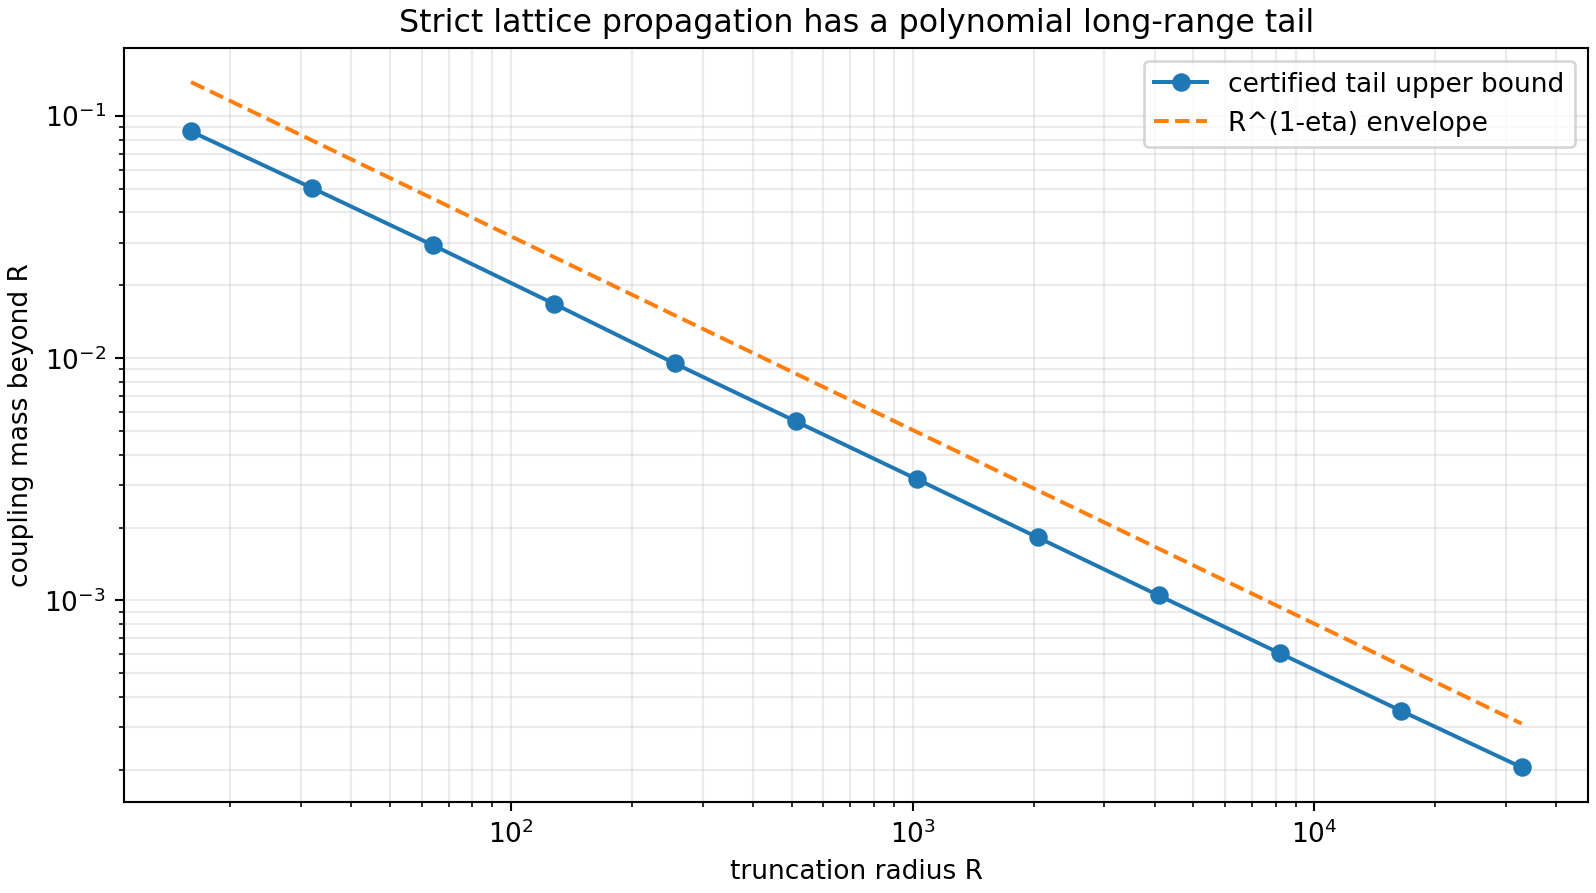
\includegraphics[width=0.92\textwidth]{FIN_Programs_91_100_Critical_Nonlocal_Operational_Figures/program94_long_range_propagation.png}
\caption{Certified coupling-tail bounds for the strict long-range lattice profile.}
\end{figure}


\section{Result}

\textbf{Theorem 94.1 --- approximate locality. \statusProven{}}

The strict absolute lattice profile admits polynomial finite-range approximations for both its unitary and diffusive dynamics, with operator error bounded by \(2|t|\tau(R)=O(|t|R^{-0.8})\).

\section{Falsification of a stronger claim}

\textbf{Claim:} the strict kernel generates an exact finite propagation cone.

\textbf{Verdict:} \textbf{\statusRefuted{}} in the stated long-range realization. The generator contains nonzero couplings at arbitrarily large distance. A strict cone would require an additional locality theorem, cancellation mechanism, or relativistic hyperbolic reconstruction not present here.

\par\medskip\hrule\medskip

\chapter{Program 95 --- Adaptive gradient flow versus quotient dynamics}

\section{Repository statement}

The adaptive moment functional is commonly written

\[
F(K)=\operatorname{tr}V(K)-\operatorname{tr}(KC),
\]

with formal evolution

\[
\dot K
=
\Pi\left[C-V'(K)\right].
\]

Program 95 asks two distinct questions:

\begin{enumerate}
\item 
Is this a gradient flow on a declared admissible operator space?

\item 
Does it descend to a regulator-free quotient under \(K\sim K+cI\)?

\end{enumerate}

\section{Projected-gradient theorem}

Let \(S\) be the linear space of real symmetric circulant matrices with zero diagonal, and let \(\Pi_S\) be the Frobenius-orthogonal projection onto \(S\). For

\[
F(K)
=
\frac a2\operatorname{tr}K^2
+\frac b4\operatorname{tr}K^4
-\operatorname{tr}(KC),
\]

the ambient gradient is

\[
\nabla F(K)=aK+bK^3-C.
\]

The constrained flow

\[
\dot K=-\Pi_S\nabla F(K)
\]

obeys

\[
\frac{dF}{dt}
=
\langle\nabla F,\dot K\rangle_F
=
-\|\Pi_S\nabla F\|_F^2
\le0.
\]

The numerical identity check gave

\[
\left|
\frac{dF}{dt}_{\mathrm{finite}}
+\|\Pi_S\nabla F\|_F^2
\right|
=5.02\times10^{-9}.
\]

\section{Quotient obstruction}

For a functional to descend to the scalar-shift quotient

\[
K\sim K+cI,
\]

it must satisfy

\[
F(K+cI)=F(K)
\]

for all admissible \(c\). The tested shifts produced defects

\[
0.214,\quad0.273,\quad4.059,\quad4.296.
\]

Thus the zero-diagonal condition is a selected constraint/\allowbreak{}slice, not a gauge quotient of this functional.

\section{Independent reproduction of P2772}

The P2772 candidate learns kernel parameters by minimizing the normalized finite \(C_{\mathrm{geo}}\) eigenclosure residual. Reproduction gives:

\begin{center}
\begingroup\small
\setlength{\tabcolsep}{3.5pt}
\renewcommand{\arraystretch}{1.16}
\begin{longtable}{@{}p{0.155\textwidth}p{0.229\textwidth}p{0.238\textwidth}p{0.238\textwidth}@{}}
\toprule
\textbf{Kernel tuple} & \textbf{loss} & \textbf{gradient norm} & \textbf{one-step loss} \\
\midrule
\endhead
legacy & 0.1130604 & 2.0011536 & 0.1091066 \\
strict & 0.04619185 & 0.08688565 & 0.04618430 \\
\bottomrule
\end{longtable}
\endgroup
\end{center}

Neither frozen tuple is stationary at tolerance \(10^{-9}\).

\section{Result}

\textbf{Theorem 95.1 --- projected law. \statusProven{}}\\
After the admissible subspace and orthogonal projection are supplied, the moment law is a genuine gradient flow and has a Lyapunov functional.

\textbf{Proposition 95.2 --- quotient claim. [Refuted in the tested nonlinear functional]}\\
The same law is not a regulator-free scalar-shift quotient flow because its functional is not invariant under \(K\mapsto K+cI\).

\textbf{P2772 fixed-point claim. [Refuted for the declared candidate]}\\
Neither frozen current kernel tuple is a fixed point of the tested \(C_{\mathrm{geo}}\)-residual learning law.

\section{Missing theorem}

A strict FIN self-learning theorem still requires:

\begin{itemize}
\item 
an ontologically sourced functional;

\item 
a declared admissible operator manifold;

\item 
a metric or mobility on that manifold;

\item 
a fixed-point or convergence theorem for the frozen tuple;

\item 
an explanation of whether diagonal/\allowbreak{}normalization conditions are constraints or true gauge redundancies.

\end{itemize}

\par\medskip\hrule\medskip

\chapter{Program 96 --- Post-P2721 strict chiral-source intake}

\section{Objective}

Program 87 constructed stable paired chiral states but did not source one branch. Since additional FAR artifacts were generated after P2721, Program 96 checks whether the exact missing input now exists.

\section{Acceptance tuple}

A candidate is admitted only if it has all five components:

\begin{enumerate}
\item 
an explicit strict formula;

\item 
a computable nonzero signed value;

\item 
non-premise provenance;

\item 
one selected P2721 coupling polarity;

\item 
robustness under the declared automorphism or gauge action.

\end{enumerate}

\section{Audited artifacts}

The following immutable inputs were checked by status and SHA-256:

\begin{itemize}
\item 
P2749: minimal inversion-odd source coupling-polarity gap;

\item 
P2750: concrete odd-source sign-value inventory no-go;

\item 
P2759: post-P2758 no-new-live-frontier reconciliation;

\item 
P2777: symmetry-source selector/\allowbreak{}geometry audit.

\end{itemize}

All four inputs are present. None exports an object satisfying all five criteria.

\section{Result}

\textbf{Proposition 96.1 --- current-source intake. [Provenance result]}

The post-P2721 material sharpens the admissible representation type and the geometric boundary, but the admitted strict signed-source count remains zero. The paired chiral dynamics remains conditional and \(QW\text{-}2191\) remains open.

\section{Why symmetry is insufficient}

An inversion-odd representation is the correct type, but it has two opposite equivariant coupling polarities. Maximal graph symmetry may distinguish a finite geometry pair, but no strict law says to maximize that quantity and it does not select \(+1\) over \(-1\) on the \(Z_{12}\) orientation orbit. Symmetry organizes degeneracy; it does not necessarily remove it.

\par\medskip\hrule\medskip

\chapter{Program 97 --- Noisy two-slot process-tensor design}

\section{Objective}

The same positive operator generates wave and diffusion:

\[
\mathcal U_t(\rho)=e^{-itL}\rho e^{itL},
\qquad
\mathcal P_t(p)=e^{-tL}p.
\]

A one-time probability can obscure their difference. A two-slot experiment inserts a recorded intermediate measurement and compares the joint intermediate/\allowbreak{}final record.

\section{Joint laws}

Starting at site \(0\), a projective site record at half-time \(\tau\) gives

\[
p_{\mathrm w}(y,z)
=
|U_\tau(y,0)|^2
|U_\tau(z,y)|^2,
\]

and

\[
p_{\mathrm d}(y,z)
=
P_\tau(y,0)
P_\tau(z,y).
\]

These are normalized two-time joint laws. The recorded intervention destroys wave coherence but is an ordinary state readout for the classical diffusion.

\section{Robust design search}

The search included:

\begin{itemize}
\item 
80 logarithmically spaced half-times from \(0.025\) to \(2\);

\item 
full-site, adjacent-pair, and parity records;

\item 
symmetric detector-confusion probabilities \(0\), \(0.05\), and \(0.10\);

\item 
a maximin Jensen--Shannon objective over detector errors.

\end{itemize}

The tested search contains 240 instrument/\allowbreak{}time designs.

\section{Best design}

The best tested maximin design is:

\[
\tau=0.9724410619973844,
\]

with full-site intermediate and final records.

Its Jensen--Shannon divergences are

\begin{center}
\begingroup\small
\setlength{\tabcolsep}{3.5pt}
\renewcommand{\arraystretch}{1.16}
\begin{longtable}{@{}p{0.420\textwidth}p{0.420\textwidth}@{}}
\toprule
\textbf{detector error} & \textbf{JS divergence} \\
\midrule
\endhead
0 & 0.210342 \\
0.05 & 0.172206 \\
0.10 & 0.151047 \\
\bottomrule
\end{longtable}
\endgroup
\end{center}

At detector error \(0.10\), the Chernoff information is

\[
C=0.1753037728.
\]

\begin{figure}[htbp]
\centering
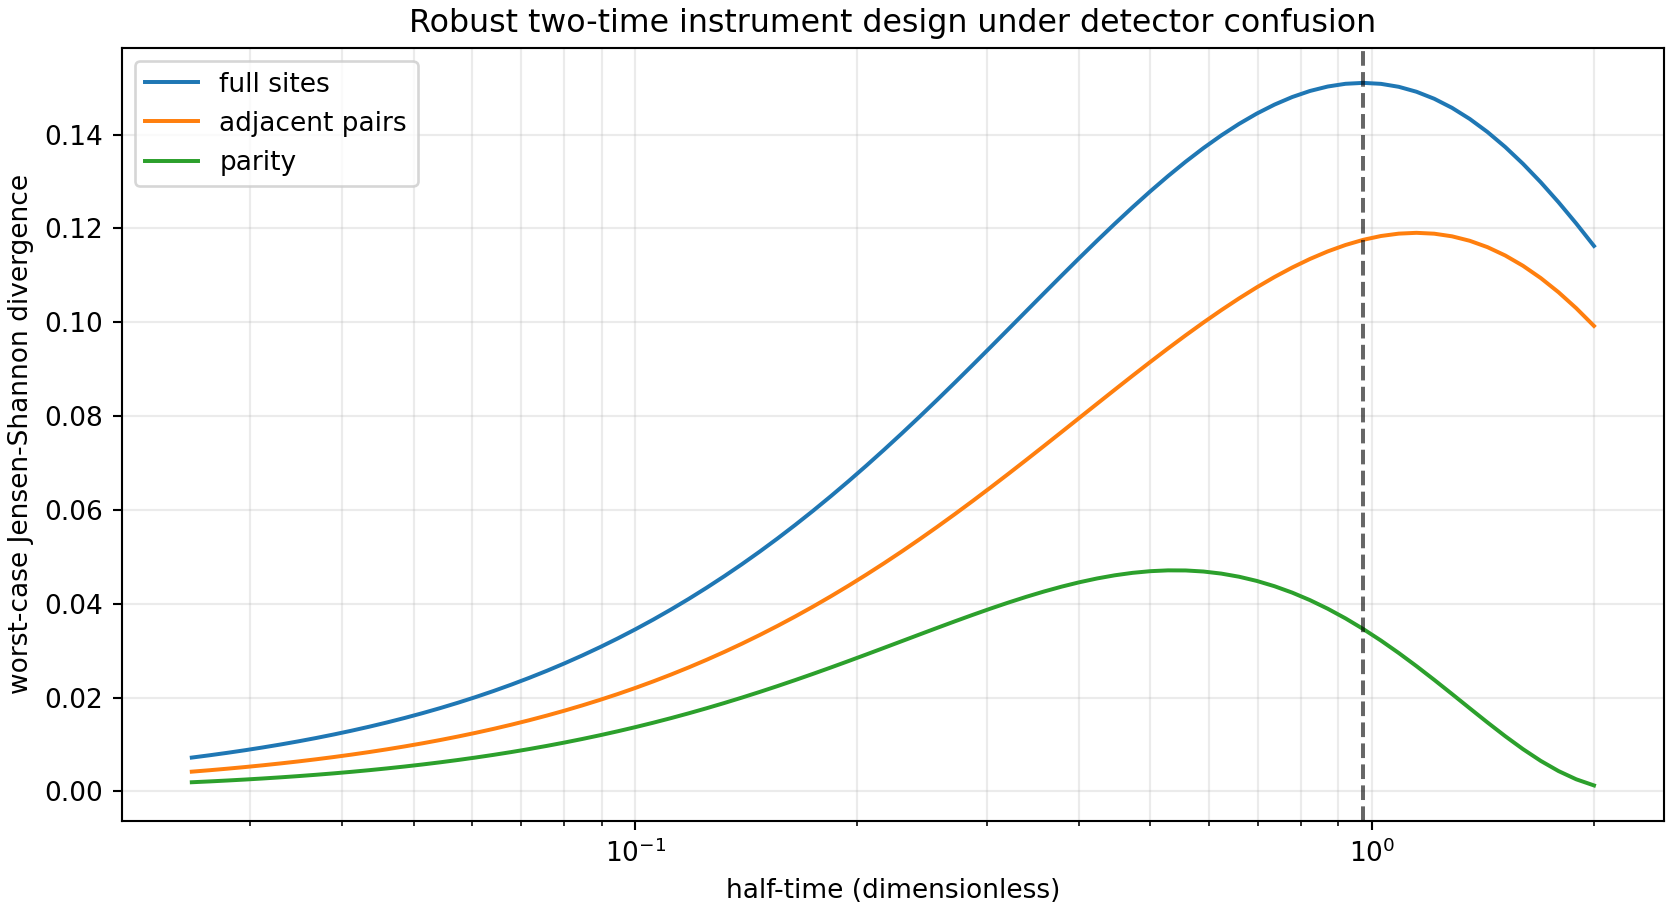
\includegraphics[width=0.92\textwidth]{FIN_Programs_91_100_Critical_Nonlocal_Operational_Figures/program97_process_tensor_design.png}
\caption{Maximin two-time instrument design under symmetric detector confusion.}
\end{figure}


\section{Monte Carlo check}

For equal priors and the exact declared model, likelihood-ratio simulations gave:

\begin{center}
\begingroup\small
\setlength{\tabcolsep}{3.5pt}
\renewcommand{\arraystretch}{1.16}
\begin{longtable}{@{}p{0.420\textwidth}p{0.420\textwidth}@{}}
\toprule
\textbf{shots} & \textbf{empirical classification error} \\
\midrule
\endhead
20 & 0.00575 \\
50 & 0 in 4000 classified samples \\
100 & 0 in 4000 classified samples \\
250 & 0 in 4000 classified samples \\
\bottomrule
\end{longtable}
\endgroup
\end{center}

Zero observed errors are not zero true error. They only indicate that the two declared finite distributions are strongly separated.

\section{Result}

\textbf{Proposition 97.1 --- robust conditional design. \statusConditional{}}

Within the declared clock range, detector model, preparation, and three instrument classes, full-site two-time records near \(\tau=0.97244\) maximize the worst-case tested wave/\allowbreak{}diffusion separation.

\section{Observer-paradox interpretation}

The operational resolution is not that an observer changes the abstract operator. Instead:

\begin{enumerate}
\item 
preparation selects an input state;

\item 
the chosen temporal semantics selects \(e^{-itL}\) or \(e^{-tL}\);

\item 
an instrument is inserted at a declared time;

\item 
the recorded intervention changes subsequent statistics;

\item 
the detector maps those records to observed data.

\end{enumerate}

The "observer" is therefore a process tester, not an unexplained metaphysical primitive. FIN still needs a theorem or axiom selecting the physical process and tester.

\par\medskip\hrule\medskip

\chapter{Program 98 --- Apparatus-inclusive feedback thermodynamics}

\section{Objective}

Program 88 verified a feedback equality. Program 98 closes the smallest memory ledger by including erasure of the outcome record.

\section{Binary measurement}

Let \(X\) be an equiprobable binary state and \(Y\) a binary symmetric measurement with error \(\epsilon\). Then

\[
I(X:Y)
=
\ln2-h(\epsilon),
\]

where

\[
h(\epsilon)
=
-\epsilon\ln\epsilon
-(1-\epsilon)\ln(1-\epsilon).
\]

The reversible feedback protocol obeys

\[
W_{\mathrm{system}}
=
\Delta F-I.
\]

The unconditional memory record has entropy

\[
H(Y)=\ln2.
\]

Resetting it in a complete cycle costs at least \(\ln2\) in the \(\beta=1\) convention. Therefore

\[
W_{\mathrm{complete}}
=
W_{\mathrm{system}}+\ln2
\]

and

\[
W_{\mathrm{complete}}-\Delta F
=
\ln2-I
=
h(\epsilon)
=
H(Y\mid X)
\ge0.
\]

All computed residuals are below \(1.2\times10^{-16}\).

\begin{figure}[htbp]
\centering
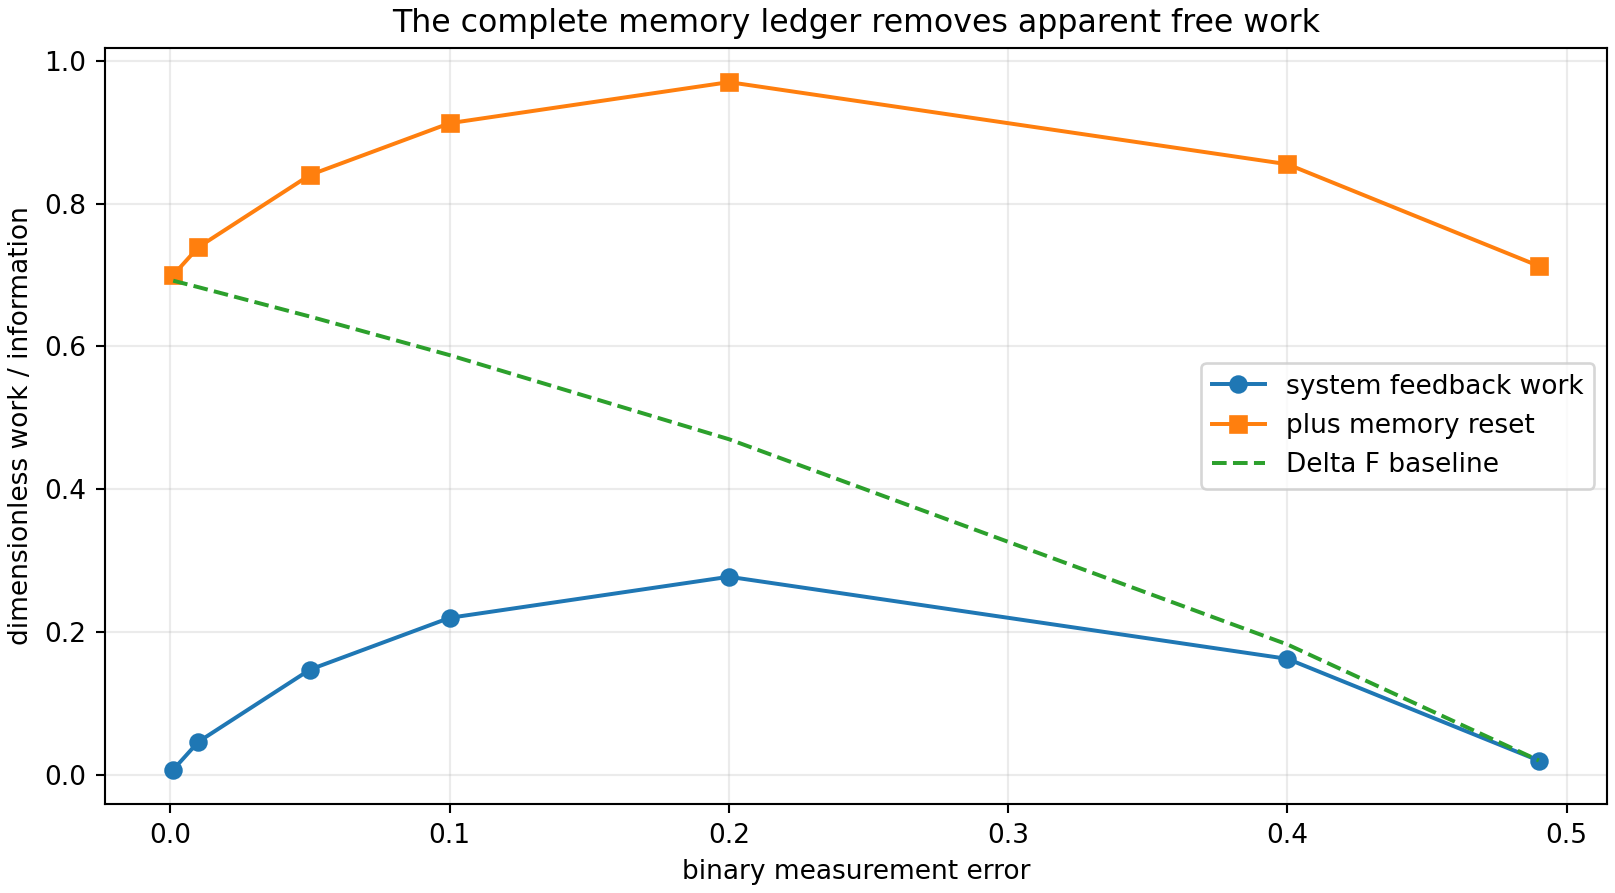
\includegraphics[width=0.92\textwidth]{FIN_Programs_91_100_Critical_Nonlocal_Operational_Figures/program98_feedback_ledger.png}
\caption{System feedback work and apparatus-inclusive work after memory reset.}
\end{figure}


\section{Result}

\textbf{Theorem 98.1 --- complete binary memory ledger. [Proven, conditional on the operational thermodynamic model]}

The apparent information-assisted reduction of system work is exactly offset in a closed apparatus cycle up to the conditional entropy:

\[
W_{\mathrm{complete}}\ge\Delta F.
\]

\section{Information-to-physics boundary}

Every quantity above is dimensionless because \(\beta=1\). A physical energy requires multiplication by a supplied thermal scale such as \(k_BT\). The kernel does not generate \(T\), \(k_B\), a bath, or the erasure apparatus. Therefore Shannon information becomes physical entropy only after a conversion package is supplied.

\par\medskip\hrule\medskip

\chapter{Program 99 --- External acquisition and power design}

\section{Objective}

No independently calibrated external dataset was admitted in Programs 81--90. Program 99 does not manufacture evidence. It turns the Program 97 distributions into a preregistered acquisition calculation.

\section{Chernoff bound}

For equal-prior i.i.d. records with distributions \(p\) and \(q\),

\[
P_{\mathrm e}^{(n)}
\le
\frac12e^{-nC(p,q)},
\]

where

\[
C(p,q)
=
-\log
\min_{0\le s\le1}
\sum_x p(x)^s q(x)^{1-s}.
\]

At the robust Program 97 design with \(10\%\) detector confusion,

\[
C=0.1753037728.
\]

Thus sufficient model-based counts are:

\begin{center}
\begingroup\small
\setlength{\tabcolsep}{3.5pt}
\renewcommand{\arraystretch}{1.16}
\begin{longtable}{@{}p{0.420\textwidth}p{0.420\textwidth}@{}}
\toprule
\textbf{target upper bound on equal-prior error} & \textbf{sufficient shots} \\
\midrule
\endhead
0.05 & 14 \\
0.01 & 23 \\
0.001 & 36 \\
0.0001 & 49 \\
\bottomrule
\end{longtable}
\endgroup
\end{center}

\section{Intake schema}

The generated intake template requires:

\begin{itemize}
\item 
immutable dataset identifier and URI;

\item 
retrieval timestamp;

\item 
license;

\item 
raw-byte SHA-256;

\item 
calibration record;

\item 
preparation and instrument definitions;

\item 
clock and unit calibration;

\item 
preregistered statistic and exclusion rule;

\item 
blind holdout identifier.

\end{itemize}

The admitted dataset list remains empty.

\section{Result}

\textbf{Proposition 99.1 --- acquisition readiness. \statusConditional{}}

The mathematical experiment now has a sample-size target and a provenance schema. It still has no external evidential input.

\par\medskip\hrule\medskip

\chapter{Program 100 --- The necessary damping-completion atom}

\section{Objective}

The legacy kernel has an asymptotically linear damping denominator, while the strict kernel uses power \(9/5\). Program 100 constructs the smallest exact pointwise atom needed to map one frozen damping envelope into the other.

\section{Frozen envelopes}

Remove oscillatory numerators and define

\[
D_{\mathrm L}(d)
=
\frac1{1+\beta_{\mathrm{tors}}d},
\qquad
\beta_{\mathrm{tors}}=0.01,
\]

and

\[
D_{\mathrm S}(d)
=
\frac1{1+\beta d^{9/5}},
\qquad
\beta=1.
\]

\section{Exact completion factor}

The pointwise positive factor satisfying

\[
D_{\mathrm S}(d)
=
C_{\mathrm{damp}}(d)D_{\mathrm L}(d)
\]

is uniquely

\[
C_{\mathrm{damp}}(d)
=
\frac{1+\beta_{\mathrm{tors}}d}
{1+\beta d^{9/5}}.
\]

The numerical reconstruction residual is

\[
2.78\times10^{-17}.
\]

\section{Asymptotic necessity}

As \(d\to\infty\),

\[
D_{\mathrm L}(d)\sim\beta_{\mathrm{tors}}^{-1}d^{-1},
\]

and

\[
D_{\mathrm S}(d)\sim\beta^{-1}d^{-9/5}.
\]

Therefore every multiplicative completion between them must satisfy

\[
C_{\mathrm{damp}}(d)
\sim
\frac{\beta_{\mathrm{tors}}}{\beta}
d^{-4/5}.
\]

A constant amplitude change or linear coordinate rescaling preserves the power-law exponent and cannot supply this atom.

The fitted tail slopes are:

\begin{center}
\begingroup\small
\setlength{\tabcolsep}{3.5pt}
\renewcommand{\arraystretch}{1.16}
\begin{longtable}{@{}p{0.420\textwidth}p{0.420\textwidth}@{}}
\toprule
\textbf{object} & \textbf{fitted slope} \\
\midrule
\endhead
legacy envelope & \(-0.99836\) \\
strict envelope & \(-1.79999999\) \\
completion multiplier & \(-0.80164\) \\
\bottomrule
\end{longtable}
\endgroup
\end{center}

\begin{figure}[htbp]
\centering
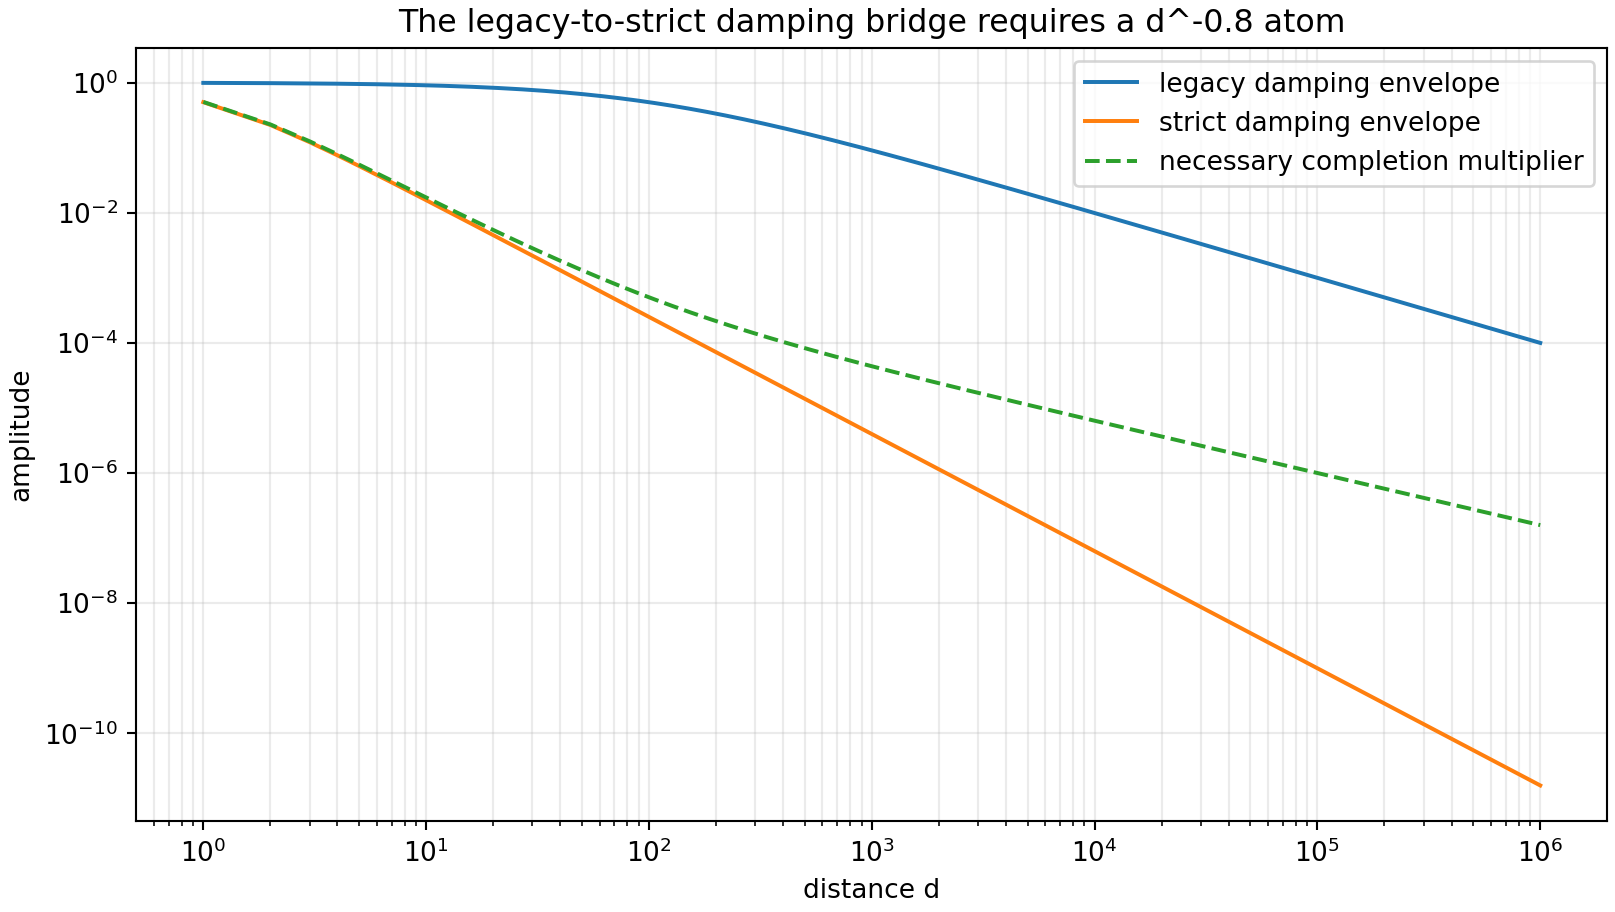
\includegraphics[width=0.92\textwidth]{FIN_Programs_91_100_Critical_Nonlocal_Operational_Figures/program100_damping_completion_atom.png}
\caption{Legacy and strict damping envelopes and their necessary \(d^{-4/5}\) completion multiplier.}
\end{figure}


\section{Result}

\textbf{Theorem 100.1 --- damping-atom necessity. \statusProven{}}

Any multiplicative legacy-to-strict damping completion must introduce asymptotic degree \(-4/5\). The displayed \(C_{\mathrm{damp}}\) is the unique positive pointwise multiplier for the two frozen denominators.

\section{Why this does not complete the bridge}

The factor is computed from both target envelopes. It therefore tells us \textbf{what a bridge must contain}, not \textbf{why FIN generates it}. It does not supply:

\begin{itemize}
\item 
a target-independent source of \(\beta=1\);

\item 
a theorem sourcing \(\eta=9/5\);

\item 
the phase/\allowbreak{}frequency passage;

\item 
the amplitude normalization passage;

\item 
the selector/\allowbreak{}topological source;

\item 
a physical-role transfer theorem.

\end{itemize}

The P2760, P2761, and P2766 provenance obstructions remain active.

\par\medskip\hrule\medskip

\chapter{Cross-program theorem inventory}

\section{Results now established}

\subsection{T91 --- strict fixed-mass nonclosure}

The infinite absolute strict lattice precision at \(m^2=1/4\) is not closed, even up to scalar normalization, under one alternating-site Schur step. \textbf{\statusComputer{}}

\subsection{T92 --- local critical prescription}

Nearest-neighbour decimation has exact ratio map \(r'=r(r+4)\). A finite local continuum mass uses \(r_N=\mu^2/N^2\); the massless kinetic coefficient needs factor-two renormalization. \textbf{\statusProven{}}

\subsection{T93 --- dense continuum classification}

Coordinate-rescaled strict matrices naturally converge to a bounded convolution operator. \textbf{[Proven formulation; strong numerical discretization evidence]}

\subsection{T94 --- polynomial approximate locality}

The strict long-range tail yields a finite-range approximation error \(O(|t|R^{-0.8})\) for both temporal semantics. \textbf{\statusProven{}}

\subsection{T95 --- projected adaptive gradient law}

Once an operator subspace and orthogonal projection are supplied, the moment law is a gradient flow. It is not automatically a quotient flow. \textbf{[Proven/\allowbreak{}refuted in declared scope]}

\subsection{T98 --- complete feedback ledger}

With memory reset included, \(W_{\mathrm{complete}}-\Delta F=H(Y\mid X)\ge0\). \textbf{[Proven, conditional]}

\subsection{T100 --- necessary damping degree}

The frozen legacy-to-strict damping multiplier has asymptotic degree \(-4/5\). \textbf{\statusProven{}}

\section{Conditional constructions}

\begin{itemize}
\item 
the two-slot wave/\allowbreak{}diffusion process tester;

\item 
its maximin clock and detector design;

\item 
Chernoff acquisition counts;

\item 
feedback thermodynamics;

\item 
the \(C_{\mathrm{damp}}\) bridge atom as a target-coded map.

\end{itemize}

\section{Still-open strict statements}

\begin{itemize}
\item 
a strict source for \(\eta=9/5\) and \(\beta=1\);

\item 
a strict signed chiral source and P2721 polarity;

\item 
a canonical dimensional scale;

\item 
a source-derived local continuum trajectory;

\item 
a physical state law and Born rule;

\item 
a Lorentzian continuum;

\item 
external empirical validation.

\end{itemize}

\par\medskip\hrule\medskip

\chapter{Failed approaches and why they failed}

\section{Frobenius convergence as continuum closure}

\textbf{Failure.} Dense rows can have \(O(N^{-1/2})\) Frobenius defects while their uniform Fourier-symbol defect remains nonzero.

\textbf{Correction.} Use scale-invariant mode ratios or uniform symbol norms. Program 91 supplies a certified ratio obstruction.

\section{Fixed positive mass as a local RG trajectory}

\textbf{Failure.} A fixed positive mass flows away from the massless local fixed shape and, in broad normalized symbol classes, toward a constant precision.

\textbf{Correction.} Tune \(m/c=O(N^{-2})\) and rescale the kinetic coefficient.

\section{Coordinate rescaling as proof of locality}

\textbf{Failure.} Coordinate rescaling yields a valid continuum operator, but its high-mode spectrum is bounded.

\textbf{Correction.} Call the result a nonlocal convolution/\allowbreak{}graphon theory unless a new singular localizing limit is proven.

\section{Long-range decay as a strict causal cone}

\textbf{Failure.} \(d^{-1.8}\) couplings are nonzero at every distance.

\textbf{Correction.} Use a polynomial approximation bound and distinguish it from finite propagation.

\section{Projecting out the diagonal as a gauge quotient}

\textbf{Failure.} The tested moment functional changes under \(K\mapsto K+cI\).

\textbf{Correction.} Treat zero diagonal as a declared constraint unless a scalar-shift invariant functional is constructed.

\section{Generic symmetry as a branch selector}

\textbf{Failure.} Inversion-odd objects and highly symmetric geometries still come with paired signs or require an unsourced optimization principle.

\textbf{Correction.} Require one formula-level signed source and one selected coupling polarity.

\section{Information-assisted work without apparatus reset}

\textbf{Failure.} Omitting the memory cycle makes mutual information look like free work.

\textbf{Correction.} Include memory creation, record, feedback, and reset in one ledger.

\section{A target-coded bridge map as a source theorem}

\textbf{Failure.} Dividing the strict envelope by the legacy envelope constructs an exact map but does not derive its parameters.

\textbf{Correction.} Use \(C_{\mathrm{damp}}\) as an obligation specification. A successful bridge still needs an independent source law.

\par\medskip\hrule\medskip

\chapter{What the present FIN object is}

\section{Best mathematical classification}

After Programs 1--100, the most robust classification is:

\begin{quote}\itshape
FIN contains a family of finite and long-range spectral operators with exact unitary/\allowbreak{}diffusive functional calculus, variational and adaptive extensions, and a partially specified operational testing layer.

\end{quote}

Its strongest natural homes are:

\begin{enumerate}
\item 
spectral operator theory;

\item 
spectral graph theory and graph signal processing;

\item 
nonlocal integral operators and graphon limits;

\item 
adaptive operator dynamics;

\item 
operational stochastic/\allowbreak{}quantum process theory.

\end{enumerate}

\section{What it is not yet}

It is not yet:

\begin{itemize}
\item 
a local relativistic field theory;

\item 
a dimensionally calibrated statistical mechanics;

\item 
a quantum theory with a derived state/\allowbreak{}Born rule;

\item 
an experimentally identified process;

\item 
a completed legacy-to-strict theory;

\item 
a closed Theory of Everything.

\end{itemize}

\section{The information interpretation}

The nadsoliton may consistently be interpreted as primordial information in a solitonic state. Mathematically, however, "information" currently labels dimensionless state/\allowbreak{}operator structure. To become experimentally meaningful physics, it still needs:

\[
\begin{aligned}
\text{dimensionless informational process}
&+\text{conversion package}\\
&+\text{sector/selector package}\\
&+\text{calibrated tester}.
\end{aligned}
\]

No single scalar entropy can replace these three logically distinct inputs.

\par\medskip\hrule\medskip

\chapter{Minimal bridge from mathematics to experiment}

The shortest currently defensible chain is:

\begin{enumerate}
\item 
\textbf{Operator:} specify a positive self-adjoint \(A\).

\item 
\textbf{Temporal semantics:} choose \(e^{-itA}\), \(e^{-tA}\), or a larger open process.

\item 
\textbf{State:} supply a normalized initial state.

\item 
\textbf{Clock:} calibrate the dimensionless parameter \(t\).

\item 
\textbf{Preparation:} specify how the state is produced.

\item 
\textbf{Instrument:} define intermediate interventions and records.

\item 
\textbf{Detector:} define confusion, efficiency, and coarse graining.

\item 
\textbf{Environment:} specify bath or memory channels.

\item 
\textbf{Units:} supply length, time, action, and temperature conversions.

\item 
\textbf{Data:} acquire independent immutable records under preregistration.

\end{enumerate}

Programs 97--99 implement items 3--7 and 10 as a conditional protocol. They do not derive those items from the kernel.

\par\medskip\hrule\medskip

\chapter{Recommended next studies: Programs 101--112}

The following recommendations are ranked by mathematical leverage, novelty relative to exhausted lanes, feasibility, and probability of producing either a theorem or a decisive no-go. Probabilities refer to obtaining a publishable mathematical result, not to confirming FIN.

\section{Program 101 --- Fully formal interval proof of T91}

\textbf{Probability of publishable result:} 0.95

Replace floating-point summation by rational or directed-rounding intervals. Prove bounds for \(Z\), \(\widehat p(\pi)\), and \(\widehat p(\pi/2)\) with a checker independent of NumPy.

\textbf{Success criterion:} a compact certificate verifiable by two independent interval libraries.

\textbf{Stop rule:} do not extend to more modes if the two-mode margin remains larger than \(10^{-2}\); the present obstruction is already sufficient.

\section{Program 102 --- Parameter-space nonclosure region}

\textbf{Probability:} 0.88

Extend the scale-invariant ratio theorem from one frozen mass to intervals in

\[
(m^2,\omega,\phi,\beta,\eta).
\]

Use interval branch-and-bound to locate any exceptional closure surface.

\textbf{Success criterion:} either an open neighborhood of certified nonclosure around the strict tuple or one explicit candidate closure locus.

\textbf{Guardrail:} a closure locus is not a FIN source theorem.

\section{Program 103 --- Graphon convergence theorem with rates}

\textbf{Probability:} 0.90

Prove operator-norm or Hilbert--Schmidt convergence of the dense coordinate-rescaled matrices to the circle convolution operator. Separate the diagonal-removal \(O(N^{-1})\) error from quadrature error.

\textbf{Success criterion:} an explicit bound

\[
\|T_N-T\|\le C/N
\]

for the strict profile or an optimal weaker rate under its regularity.

\section{Program 104 --- Search for a singular localizing limit}

\textbf{Probability:} 0.62

Test rescaled kernels

\[
g_\varepsilon(x)
=
\varepsilon^{-1}g(x/\varepsilon)
\]

and centered second-moment generators to determine whether a local Laplacian, fractional Laplacian, or neither emerges.

\textbf{Success criterion:} Mosco/\allowbreak{}resolvent convergence to a declared differential or fractional operator.

\textbf{Stop rule:} if the required rescaling is arbitrary and not sourced, record it as a conversion axiom, not strict FIN output.

\section{Program 105 --- Fractional-tail universality}

\textbf{Probability:} 0.84

Remove the oscillatory absolute-value modulation analytically and determine whether the small-\(q\) lattice symbol has

\[
1-\widehat p(q)\asymp |q|^{\eta-1}=|q|^{0.8}.
\]

This would identify the long-range lattice route with a fractional generator of order \(0.8\), subject to modulation constants.

\textbf{Success criterion:} matching upper and lower Tauberian bounds.

\section{Program 106 --- Sharp long-range Lieb--Robinson comparison}

\textbf{Probability:} 0.78

Compare the Program 94 Duhamel bound with modern long-range propagation bounds. Determine the strongest polynomial or stretched cone available for one-particle and many-body lifts.

\textbf{Success criterion:} a theorem with explicit exponent and constants for the strict \(d^{-1.8}\) tail.

\textbf{Guardrail:} do not call a polynomial light cone Lorentz invariance.

\section{Program 107 --- Adaptive-manifold geometry}

\textbf{Probability:} 0.80

Define the admissible kernel manifold explicitly, including positivity, normalization, symmetry, and parameter constraints. Compare Euclidean, Fisher, and affine-invariant metrics for

\[
\dot K=-\operatorname{grad}_gF.
\]

\textbf{Success criterion:} a well-posed gradient flow and a proof of invariance of the admissible cone.

\textbf{Stop rule:} no "self-learning nadsoliton" claim until the functional is ontologically sourced.

\section{Program 108 --- Source functional for the frozen kernel tuple}

\textbf{Probability:} 0.45

Attempt an inverse variational problem: find the lowest-complexity functional whose stationary equations contain the frozen strict tuple without explicitly encoding that tuple as a target.

\textbf{Success criterion:} a source law satisfying identifiability and out-of-sample parameter prediction.

\textbf{Falsification:} minimum-description-length comparison against a direct four-parameter fit.

\section{Program 109 --- Chiral-source acceptance test}

\textbf{Probability:} 0.25 without new input; 0.75 after a real candidate is supplied

Do not enumerate more names. Admit only one new formula carrying a nonzero signed value and an explicit P2721 polarity coupling, then run the five-part Program 96 gate.

\textbf{Success criterion:} all five criteria pass.

\textbf{Stop rule:} if no new formula is supplied, preserve the no-source certificate and do not replay the lane.

\section{Program 110 --- Experimental process-tensor preregistration}

\textbf{Probability:} 0.85 for a complete protocol

Turn Program 97 into a frozen preregistration:

\begin{itemize}
\item 
clock grid;

\item 
preparation;

\item 
full-site instrument;

\item 
detector confusion estimator;

\item 
primary log-likelihood statistic;

\item 
blind holdout;

\item 
exclusion rules;

\item 
calibration uncertainty.

\end{itemize}

\textbf{Success criterion:} an immutable protocol ready before data access.

\section{Program 111 --- Apparatus thermodynamics beyond the binary idealization}

\textbf{Probability:} 0.82

Add finite-time control, nonzero dissipation, detector memory, and correlated errors. Prove a complete entropy-production inequality for the joint system--controller--record process.

\textbf{Success criterion:} a path-space fluctuation relation with every memory register included.

\section{\texorpdfstring{Program 112 --- Source theorem for the \(-4/5\) damping atom}{Program 112 --- Source theorem for the -4/\allowbreak{}5 damping atom}}

\textbf{Probability:} 0.35

Seek one target-independent mechanism whose scaling dimension is \(-4/5\) and which couples the legacy denominator to the strict compression law. Candidate mathematical routes include a fractional fixed point, multiplicative cascade, or anomalous dimension, but the exponent must be predicted rather than inserted.

\textbf{Success criterion:} derive \(\eta=9/5\), \(\beta>0\), and the completion factor from premises that do not contain the strict target values.

\textbf{Stop rule:} if the exponent is fitted or copied into the premise, classify the result as parametrization, not a bridge theorem.

\par\medskip\hrule\medskip

\chapter{Ranked roadmap}

\begin{center}
\begingroup\small
\setlength{\tabcolsep}{3.5pt}
\renewcommand{\arraystretch}{1.16}
\begin{longtable}{@{}p{0.081\textwidth}p{0.142\textwidth}p{0.414\textwidth}p{0.223\textwidth}@{}}
\toprule
\textbf{Rank} & \textbf{Program} & \textbf{Expected value} & \textbf{Probability} \\
\midrule
\endhead
1 & 101 & Turns the main new obstruction into independently checkable theorem data & 0.95 \\
2 & 103 & Gives the natural dense continuum route a rigorous analytic identity & 0.90 \\
3 & 102 & Determines robustness or exceptional closure loci & 0.88 \\
4 & 105 & May identify the lattice route with a fractional universality class & 0.84 \\
5 & 107 & Makes adaptive dynamics mathematically intrinsic to an admissible manifold & 0.80 \\
6 & 106 & Sharpens propagation without false Lorentz claims & 0.78 \\
7 & 110 & Makes the operational test genuinely preregisterable & 0.85 \\
8 & 111 & Completes thermodynamics beyond the reversible binary toy model & 0.82 \\
9 & 104 & Tests whether locality can emerge through a singular limit & 0.62 \\
10 & 108 & Attempts a non-target-coded learning source & 0.45 \\
11 & 112 & Attempts to source the missing damping anomalous dimension & 0.35 \\
12 & 109 & Only valuable after one genuinely new signed source is supplied & 0.25 \\
\bottomrule
\end{longtable}
\endgroup
\end{center}

The recommended execution order is:

\[
101
\rightarrow
103
\rightarrow
102
\rightarrow
105
\rightarrow
107
\rightarrow
106
\rightarrow
110
\rightarrow
111,
\]

with Programs 104, 108, 109, and 112 gated by explicit new premises.

\par\medskip\hrule\medskip

\chapter{Final scientific judgment}

The present round changes the status of one major question. The strict lattice nonclosure is no longer merely a large-\(N\) numerical suspicion. In the declared positive precision realization at \(m^2=1/4\), it follows from an exact Schur alias law and an explicit tail certificate.

At the same time, the continuum problem becomes clearer rather than less favorable. FIN does possess a natural continuum interpretation: the dense coordinate-scaled route converges to a bounded nonlocal convolution operator. What it does not possess automatically is a local relativistic field theory. The local route exists mathematically only after critical mass tuning and operator renormalization are supplied as scale-dependent data.

The wave/\allowbreak{}diffusion pair remains one of the strongest structural features. Program 97 shows how an observer/\allowbreak{}apparatus can be modeled operationally as a two-slot tester and how the two temporal semantics can be distinguished even with detector confusion. Program 98 shows why this does not turn Shannon information into free energy: the apparatus record and reset complete the ledger.

The smallest new bridge object is also now explicit. The legacy-to-strict damping passage requires an asymptotic \(d^{-4/5}\) multiplier. This is a real mathematical obligation, but not yet an explanation: the repository still lacks a source theorem for that anomalous degree, for \(\beta=1\), and for the strict phase data.

The deepest interpretation surviving this round is therefore:

\begin{quote}\itshape
FIN is a mathematically coherent spectral and adaptive nonlocal operator framework whose unitary and diffusive shadows admit an operational process theory. Its natural dense continuum is a bounded integral operator; a local physical continuum, dimensional calibration, strict selector, measurement law, and legacy-to-strict source theorem remain additional structures.

\end{quote}

This conclusion is neither a rejection nor a confirmation of a physical FIN theory. It is the strongest statement that survives the present falsification tests.

\par\medskip\hrule\medskip

\chapter{Appendix A --- Exact formulas used in the computation}

\section{A.1 Strict lattice normalization}

\[
a_d
=
\frac{|\cos(0.18575d+0.16250)|}{1+d^{1.8}},
\qquad
Z=2\sum_{d\ge1}a_d.
\]

\section{A.2 Symbol}

\[
\widehat p(q)
=
\frac2Z\sum_{d\ge1}a_d\cos(qd),
\qquad
\lambda(q)=m^2+1-\widehat p(q).
\]

\section{A.3 Harmonic alias}

\[
\lambda_{\mathrm S}(\theta)
=
\frac{
2\lambda(\theta/2)\lambda(\theta/2+\pi)
}{
\lambda(\theta/2)+\lambda(\theta/2+\pi)
}.
\]

\section{A.4 Nearest-neighbour decimation}

\[
c'=\frac{c^2}{m+2c},
\qquad
m'=\frac{m(m+4c)}{m+2c}.
\]

\section{A.5 Nonlocal continuum precision}

\[
A=m^2I+I-T,
\qquad
(Tf)(x)
=
Z^{-1}\int_0^1g(x-y)f(y)\,dy.
\]

\section{A.6 Propagators}

\[
U_t=e^{-itA},
\qquad
P_t=e^{-tA}.
\]

\section{A.7 Adaptive moment functional}

\[
F(K)
=
\frac a2\operatorname{tr}K^2
+\frac b4\operatorname{tr}K^4
-\operatorname{tr}(KC).
\]

\section{A.8 Damping completion}

\[
C_{\mathrm{damp}}(d)
=
\frac{1+0.01d}{1+d^{9/5}}.
\]

\par\medskip\hrule\medskip

\chapter{Appendix B --- Reproducibility files}

\begin{itemize}
\item 
FIN\_Programs\_91\_100\_Critical\_Nonlocal\_Operational\_Monograph.md

\item 
FIN\_Programs\_91\_100\_Critical\_Nonlocal\_Operational\_Monograph.tex

\item 
FIN\_Programs\_91\_100\_Critical\_Nonlocal\_Operational\_Monograph.pdf

\item 
\path{fin_programs_91_100_critical_nonlocal_operational.py}

\item 
test\_\path{fin_programs_91_100_critical_nonlocal_operational.py}

\item 
\path{FIN_Programs_91_100_Critical_Nonlocal_Operational_Results.json}

\item 
\path{FIN_Programs_91_100_External_Data_Intake_Template.json}

\item 
\path{FIN_Programs_91_100_Critical_Nonlocal_Operational_Figures/}

\end{itemize}

The executable uses the deterministic seed \(20260727\). The main theorem in Program 91 does not rely on random sampling.

\par\medskip\hrule\medskip

\chapter{Appendix C --- Release guardrail}

This release does not:

\begin{itemize}
\item 
identify the strict and legacy kernels as raw equal objects;

\item 
transfer \(\sin^2\theta_W=\alpha_{\mathrm{geo}}/12\), \(\alpha_{\mathrm{EM}}^{-1}\), or a \(\beta^N\) hierarchy to the strict kernel;

\item 
discharge \(QW\text{-}2191\);

\item 
derive a dimensional standard;

\item 
derive a Born rule;

\item 
prove Lorentz invariance;

\item 
promote a role-bearing \(L_{\mathrm{total}}\);

\item 
claim a completed Theory of Everything;

\item 
claim external empirical support.

\end{itemize}

The exact output is narrower and stronger: ten declared mathematical and operational studies, with positive theorems, explicit counterexamples, conditional constructions, and preserved open boundaries.


\clearpage
\chapter*{Archival note}
\addcontentsline{toc}{chapter}{Archival note}
Machine-readable results are stored in
\path{FIN_Programs_91_100_Critical_Nonlocal_Operational_Results.json}.
The executable, seventeen tests, seven figures, and external-data intake
template reproduce the release.

\medskip
\noindent\textbf{Suggested citation:}

\.Zuchowski, K. (2026). \emph{FIN Programs 91--100: Critical Scaling,
Nonlocal Continuum Structure, and Operational Completion Tests}
(FIN Research Monograph, Release 10.10; Version 1.0.0) [Preprint].
\end{document}
